\documentclass[onecolumn,10pt,titlepage]{article}
\usepackage[a4paper,top=2.5cm,bottom=2cm,left=2cm,right=2cm,marginparwidth=1.75cm,headheight=28pt]{geometry}
\usepackage[utf8]{inputenc}
\usepackage[spanish,mexico]{babel} 
\usepackage{natbib}
\usepackage[symbol]{footmisc}
\renewcommand*{\thefootnote}{\fnsymbol{footnote}}
% \renewcommand{\thefootnote}{\fnsymbol{footnote}}
% \footnote[num]{text}

% \pagestyle{myheading}
% \markright{Mi Documento \hfill Mi nombre \hfi}
\usepackage{fancyhdr,framed}
\setlength{\headheight}{15.2pt}
\pagestyle{fancy}
\lhead{Elementos Finitos II - 31.92 \\ Patricio Whittingslow -- 55423}
\chead{TP 1}

\usepackage{caption}
\usepackage{subcaption}
\usepackage{amsmath}

\usepackage{multicol}
%\usepackage{mathastext} %BORRAR O DEJAR: Cambia estilo de la fuente matemática y la deja con aspecto mas "técnico".
\usepackage{graphicx}
\usepackage{hyperref}
\hypersetup{
    colorlinks,
    citecolor=black,
    filecolor=black,
    linkcolor=black,
    urlcolor=black
}

%Helvetica
\renewcommand{\familydefault}{\sfdefault}
\usepackage[scaled=1]{helvet}
\usepackage[format=plain,
            labelfont={bf,it},
            textfont=it]{caption}
%--------------------------------------



%\usepackage{siunitx}
\newcommand{\glossentry}[2]{$#1$ \indent #2 \par \vspace{.4cm} }
\newcommand{\adm}{\textrm{adm}}
\newcommand{\unit}[1]{\textsf{#1}}
\newcommand{\mega}{\unit{M}}
\newcommand{\milli}{\unit{m}}
\newcommand{\giga}{\unit{G}}
\newcommand{\meter}{\unit{m}}
\newcommand{\pascal}{\unit{Pa}}
\newcommand{\kilo}{\unit{k}}
\newcommand{\si}[1]{#1}
\newcommand{\SI}[2]{#1\si{#2}}
\title{Informe Técnico - ITBA}

\author{Patricio Whittingslow}
%========================> Comienza Documento
\begin{document}
\begin{titlepage}
	\centering
	
	{ \large Instituto Tecnológico de Buenos Aires  \par }
	\vspace{2cm}
	{\Large \scshape Elementos Finitos II - 31.92 \par}
	\vspace{2cm}
	{\Huge \scshape Estudio del Doble Fondo de un Buque\par }
	\vspace{.5cm}
	{\Large Y porque una placa no es una cascara plana \par}
	\vspace{2cm}
	{\large \bf Autor \par}
	\vspace{.5cm}
	\textsc{\large Patricio Whittingslow -- 55423}
	\vspace{2cm}
	{\par \large Fecha de realización: \today \par}
	\vspace{1cm}
	{\large Fecha de entrega: .......................................\par}
	\vspace{2.5cm}
	{\large Firma del docente: .......................................}
	\vspace{3cm}
	\begin{figure}[htb!]
		\centering
		
\includegraphics[width=6cm]{logoitba.png}
	\end{figure}
\end{titlepage}


{\textbf{Problema}}\par
Se estudia la estructura de la base de un buque empleando el uso del método de elementos finitos. Las hipótesis empleadas son de desplazamientos pequeños y material isótropo.

\begin{multicols}{2}
	\section*{Glosario}
	\glossentry{F}{Rigidez ante la flexión.}
	\glossentry{p}{Carga de presión.}
	%\glossentry{x}{}
\end{multicols}


\tableofcontents


\section{Introducción Teórica}
Se optó por resolver el problema con elementos cascaras de 4 nodos y elementos vigas. Antes de comenzar a modelar se estudió el funcionamiento de los elementos placas (Mindlin y Kirchoff) para tener un concepto fundado de como se pueden emplear y cual es su comportamiento ante casos empotrados y articulados.

En el estudio de placas con pequeñas deformaciones en general toma en cuenta las siguientes suposiciones\cite{ugural2003advanced}

\begin{enumerate}
	\item La relación entre el espesor de la cascara al radio de curvatura es mucho menor a la unidad
	\item Desplazamientos son muy pequeños en comparación con el espesor
	\item Secciones rectas de un elementos, perpendiculares al plano medio, permanecen rectas y perpendiculares al plano \textit{deformado}.
	\item Se desprecia $\sigma_z$ (al igual que en placas).
\end{enumerate}

Se entiende un elemento cascara como un elemento con poco espesor de tal forma que no tiene tensiones por corte o flexión. En un elemento placa dominan estas tensiones. 


\subsection{Estudio con placas planas}
Las placas a estudiar son del tipo que se puede encontrar en cualquier bilbiografía que trate elasticidad\cite{ugural2003advanced}. Las tensiones estan dadas por 

\begin{align} \sigma_{x} &=\frac{E}{1-v^{2}}\left(\varepsilon_{x}+v \varepsilon_{y}\right)=-\frac{E z}{1-v^{2}}\left(\frac{\partial^{2} w}{\partial x^{2}}+v \frac{\partial^{2} w}{\partial y^{2}}\right) \\ \sigma_{y} &=\frac{E}{1-v^{2}}\left(\varepsilon_{y}+v \varepsilon_{x}\right)=-\frac{E z}{1-v^{2}}\left(\frac{\partial^{2} w}{\partial y^{2}}+v \frac{\partial^{2} w}{\partial x^{2}}\right) \\ \tau_{x y} &=\frac{E}{2(1+v)} \gamma_{x y}=-\frac{E z}{1+v} \frac{\partial^{2} w}{\partial x \partial y} 
\end{align}
lo que nos dice que las tensiones varían linealmente sobre el espesor de la placa (en $z$), lo que va ser importante para aclarar algunas cosas mas tarde.


El problema trata una placa de espesor $t$ con dimensiones $a\times b$ donde $a=1,4\si{\meter}$ y $b=1\si{\meter}$. El material es acero\footnote{$E=\SI{210}{\giga \pascal}$ y $\nu=0,3$}. Los casos son con presión uniforme $p$ para los espesores $t=a$, $t=\frac{a}{10}$ y $t=\frac{a}{100}$ usando elementos Kirchoff Q4 y Mindlin Q8. El factor de corrección para tensión por corte transverso es igual a $k=\frac{5}{6}$ usando integración selecta\citep{cook2007concepts} para placas Mindlin . 

Los resultados se comparan con la solución analítica para una placa simplemente apoyada\citep{ugural2003advanced}\footnote{Utilizando $n=m=9$ dado que convergía bien para ese número de iteraciones.}. Para los casos estudiados el desplazamiento máximo es $w_{\max}(t)\approx \SI{6,71e-9}{\meter}$, $w_{\max}(0,1t)\approx \SI{6,71e-6}{\meter}$, $w_{\max}(0,01t)\approx \SI{6,71e-3}{\meter}$. Como sería de esperar, hay una relación del tipo $w(t)=Ct^3$. Para el caso empotrado no se considera solución analítica debido a la inaccesibilidad de los artículos que trataban una solución. 
\begin{table}[htb!] 
	\centering
	\begin{tabular}{clll}
		Número de Elementos& Kirchoff & Mindlin Q4 & Mindlin Q8  \\ \hline
		60  & \SI{1,758}{\milli \meter}  &  \SI{1,869}{\milli \meter}  & \SI{1,955}{\milli \meter} \\
		280  & \SI{1,919}{\milli \meter}  &  \SI{1,950}{\milli \meter}  & \SI{1,966}{\milli \meter} \\
		4800 &\SI{1,957}{\milli \meter}  &   \SI{1,965}{\milli \meter} &\SI{1,966}{\milli \meter} \\
		15552 &  \SI{1,959}{\milli \meter}   &  \SI{1,965}{\milli \meter}  & \SI{1,966}{\milli \meter}\\
		21600&  \SI{1,959}{\milli \meter}& \SI{1,965}{\milli \meter}  & \SI{1,966}{\milli \meter}
	\end{tabular}\
	\caption{Desplazamientos máximos para carga uniforme $p=\SI{5}{\kilo \pascal}$ sobre placa con espesor $t=\frac{a}{100}$. Relación de aspecto de elementos 4:3. Utilizando integración selecta\citep{cook2007concepts}, el más costoso numéricamente por elemento fue Mindlin Q8 por un margen considerable.}
	\label{tab:Convergencia}
\end{table}



\subsection{Resultados de estudio con placas planas}
A raíz del cuadro \ref{tab:Convergencia} se puede inferir que los elementos Q8 son los mejores elementos para captar desplazamientos con un menor número de elementos. Tomando esto en cuenta y además que permiten una implementación isoparamétrica simple; se entiende por que las placas Kirchoff no aparecen en programas de elementos finitos.

Los resultados indican que las placas Mindlin se comportan bien para espesores menores, efectivamente reduciendo el error relativo. Si se refina se obtienen mejores resultados.

Las placas Kirchoff en cambio no exhiben mejora del error relativo con el cambio del espesor y convergen con poco refinamiento. Esto se debe a la libertad de deformación del elemento Kirchoff, permitiendo deformaciones del orden cubico para cada elemento.




 \begin{figure}[htb!]
 \centering
 \begin{subfigure}{0.49\textwidth}
 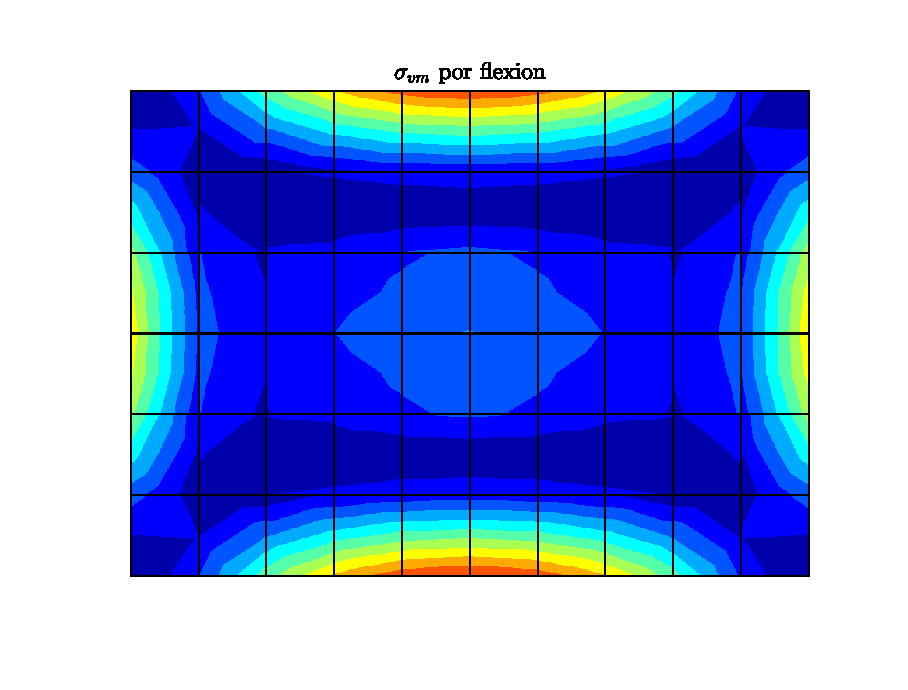
\includegraphics[width=\linewidth]{fig/VM.eps}
 \caption{Caso empotrado}
 \label{fig:VMempotrado}
 \end{subfigure}
 \begin{subfigure}{0.49\textwidth}
 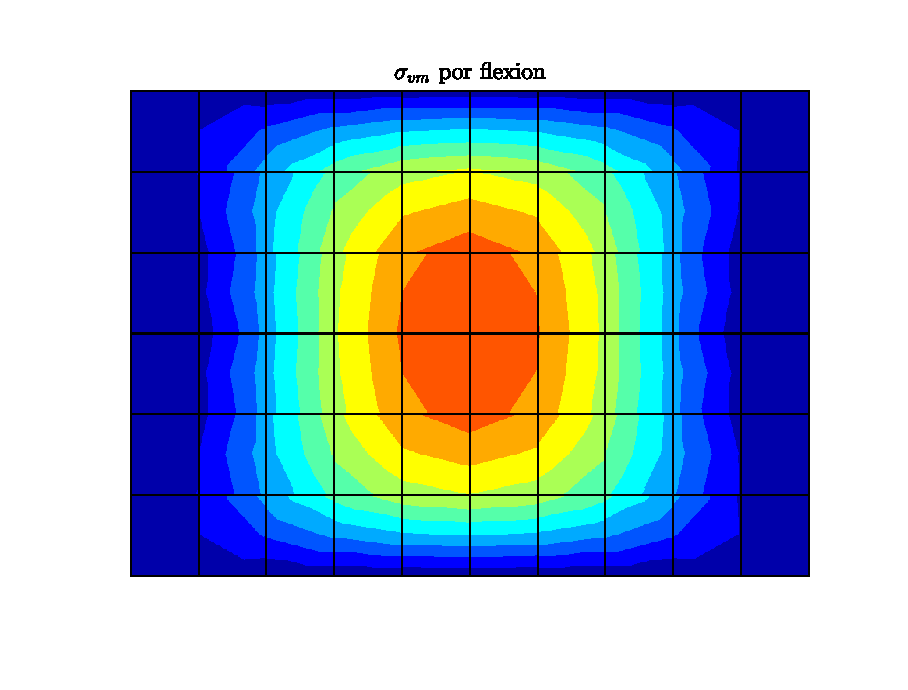
\includegraphics[width=\linewidth]{fig/VMapoyado.eps}
 \caption{Caso simplemente apoyado}
 \label{fig:VMapoyado}
 \end{subfigure}
 \caption{Tensiones calculadas de Von Mises para elementos Q8. Divisiones de elementos visible. Tensiones en Pascales. Se puede observar claramente el comportamiento diferente ante la restricción de giro. Un caso empotrado sufre de flexión en sus bordes mientras que la placa apoyada va fallar por corte.}
 \label{fig:VM}
 \end{figure}

\section{Estudio de doble fondo de un buque}
El buque a estudiar tendrá 5 metros de calado, dándonos una presión sobre el doble fondo de alrededor de $p=5 \si{\kilo \pascal}$. Esta va ser la presión nominal para la cual se va resolver el problema. Debido a la acción ondulatoria de las olas\footnote{Conocido como esfuerzos de quebranto.} el buque en realidad puede ser sometido a una presión aún mayor, por eso se va tomar un factor de seguridad $n=3$ para cuando se optimize. Se van a modelar 4 claras (distancia entre varengas) y una vagra. Las longitudinales van a ser perfiles bulbo $280\times13\si{\milli \meter}$, $300\times 13 \si{\milli \meter}$ para el fondo y el doble fondo, respectivamente. La distancia entre varengas es de $3,25\si{\meter}$ y la distancia entre vagras $4,4\si{\meter}$. Como no se dispones de perfiles bulbo en el programa a usar (NX 11.0 de Siemens) se utilizarán perfiles ``L"{} de características similares. Las dimensiones de los perfiles L se obtuvieron para que los momentos de Inercia $I_z$, $I_y$ sean lo más similares. Se utilizó WRESC\footnote{Whittingslow's Rapid Empirical Section Correlation for bulb-L.} para obtener el perfil adecuado para cada bulbo:

\begin{equation} \label{eq:WREC}
c = \frac{L}{6,25}  \qquad\qquad d \approx \frac{15,25c}{\sqrt{L}} \qquad \textrm{unidades consistentes}
\end{equation}
donde $c$ es el espesor del tramo largo (\SI{13}{\milli \meter} en este caso) mas el sobresaliente del perfil ``L"{} similar. $d$ es el espesor del sobresaliente. $L$ es la longitud identificadora del perfil bulbo. Ecuación verificada para un rango acotado de perfiles bulbo de espesor $13\si{\milli\meter}$.


\subsection{Método}
Se planteo un modelo aprovechando el eje longitudinal simétrico y considerando simetría transversal. Cabe destacar que debido a esta última consideración puede haber discrepancia entre la realidad y lo que se plantea. Es decir, \emph{considerar simetría sobre un eje transversal tomando en cuenta solo 4 claras de distancia es una decisión valida si los esfuerzos se normalizan en magnitud acercándose al borde sin soporte en $z$.\footnote{Se explica a que se refiere con el borde sin soporte en $z$ a continuación.} Caso contrario se debería tomar aún más claras para ver las tensiones mayores que se pueden llegar a alcanzar.}

La simetría es aplicada de forma que se vean esfuerzos generados por el equilibrio entre las dos fuerzas predominantes en un buque, el peso y la presión hidrostática. Para lograr esto se aplican condiciones de borde de simetría en todos los bordes del modelo y una condición especial en un borde transversal y otro longitudinal. La condición a aplicar es un soporte en la dirección de la gravedad, en este caso, un soporte en $z$. Esto dará luz al efecto ``reacción"{} del peso propio del buque ante la presión hidrostática.



 \begin{figure}[htb!]
     \centering
     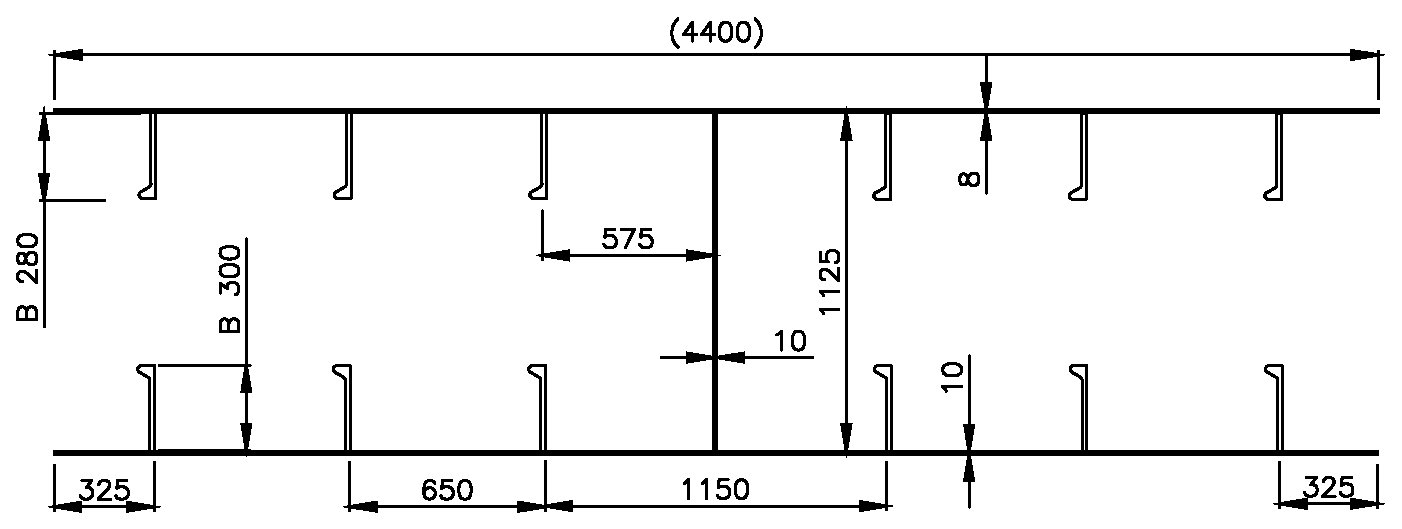
\includegraphics[width=0.7\linewidth]{fig/MODELO.eps}
     \caption{Corte transversal del modelo. La placa superior es el fondo y por el medio queda la vagra. La profundidad (longitud) del modelo es de \SI{16,25}{\meter}.}
     \label{fig:modeloTransversal}
 \end{figure}



\subsection{Resultados y optimización}
Como se puede ver, los esfuerzos se regularizan al acercarse al borde transversal sin soporte en $z$, lo cual nos da una idea que la situación vista en la figura \ref{fig:2a} podría estar ocurriendo en el interior de un buque. Lo que puede llegar a llamar la atención es que las tensiones son relativamente bajas en los longitudinales.


 \begin{figure}[htb!]
 \centering
 \begin{subfigure}{0.49\textwidth}
 % \begingroup
 \begin{framed}
 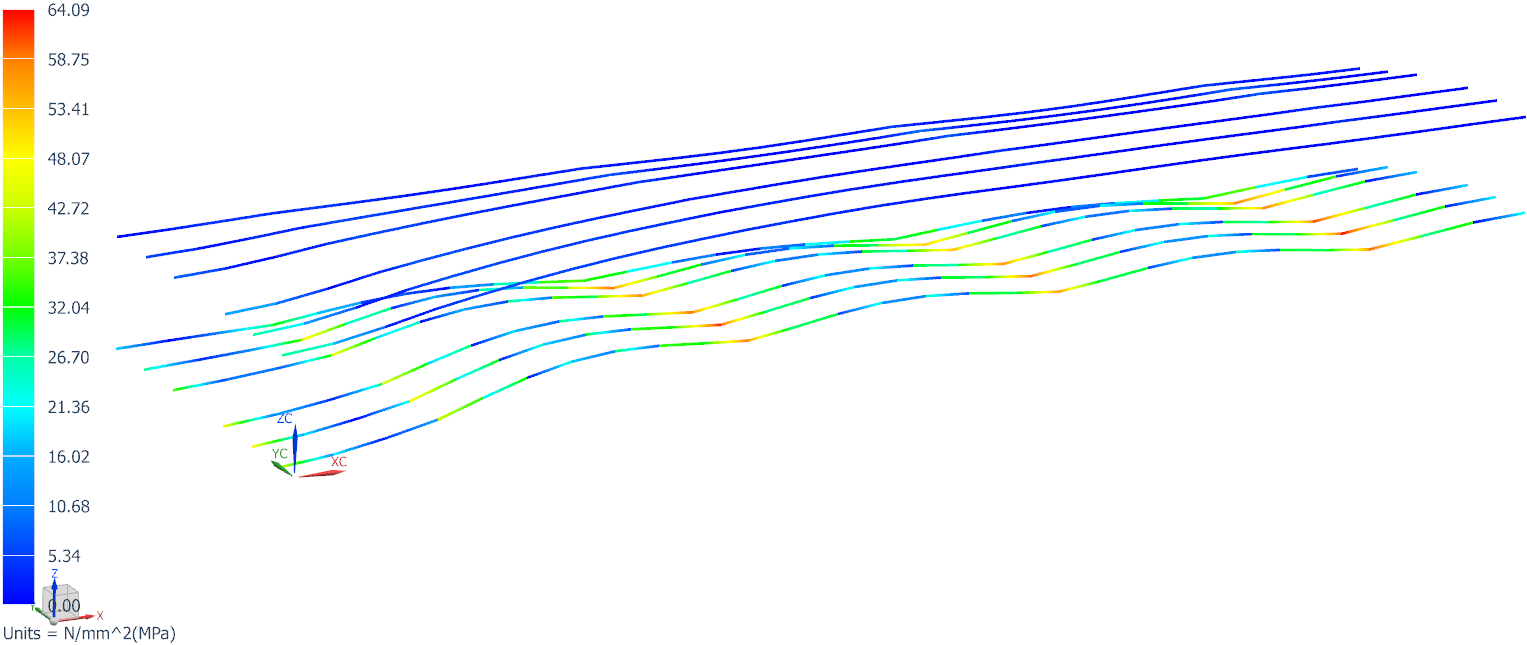
\includegraphics[height=3.3cm]{fig/longitudinales_a.png}
 \caption{Vista de los elementos viga. Perfiles superiores son los $280\times 13\si{\milli \meter}$. $\sigma_{vm_{\max}}= 64,09 $\si{\mega \pascal}.}
 \label{fig:longitudinalesCasoA}
 \end{framed}
 % \endgroup
 \end{subfigure}
 \begin{subfigure}{0.49\textwidth}
 \begin{framed}
 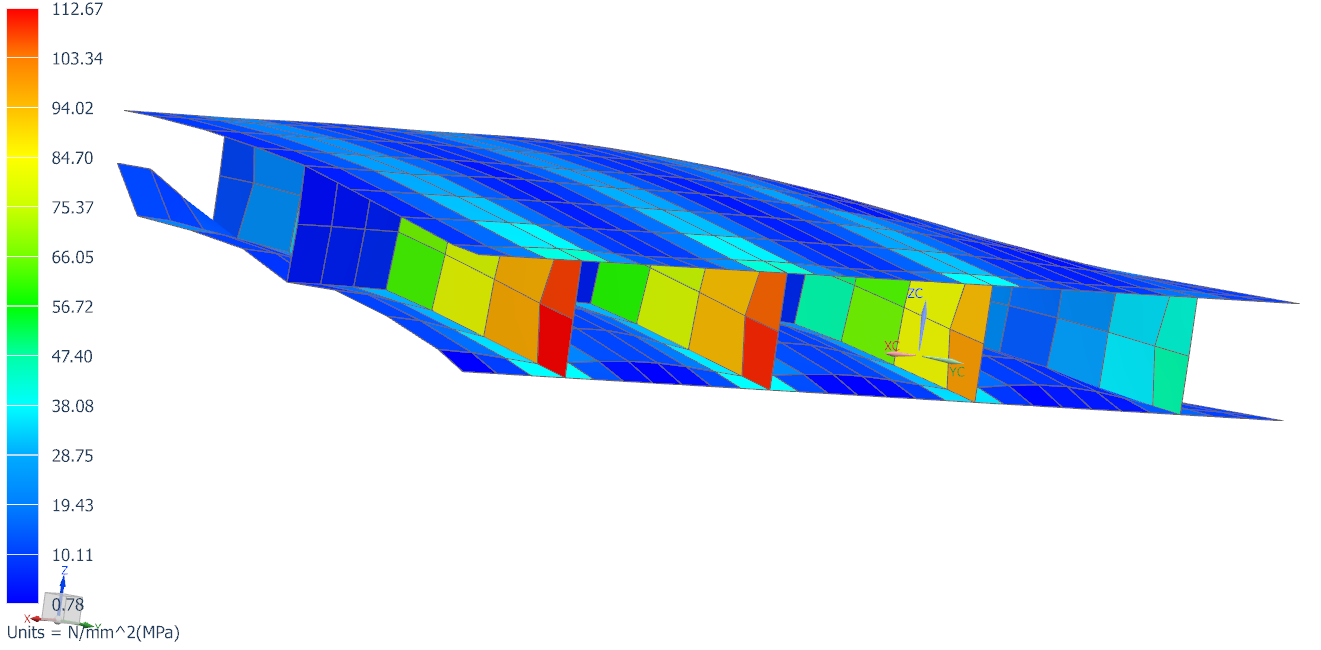
\includegraphics[height=3.3cm]{fig/varengas_a.png}
 \caption{Vista de los elementos cascaras del doble fondo. $\sigma_{vm_{\max}}= 112,67 $\si{\mega \pascal}.}
 \label{fig:VarengasCasoA}
 \end{framed}
 \end{subfigure}
 \caption{Tensiones máximas Von Mises en \si{\mega \pascal}.}
 \label{fig:2a}
 \end{figure}

\subsubsection*{Proceso de optimización}
El material a usar para todos los elementos es el acero AISI 4340 \emph{annealed} con una tensión admisible de \SI{470}{\mega \pascal}.

El proceso de optimización fue iterativo, cambiando los espesores de las vagras, varengas y fondos hasta que todos tengan una zona que este cerca de $\sigma_{\adm}=\frac{\sigma_{y}}{n}\approx\SI{150}{\mega \pascal}$. También se redujeron las secciones de las longitudinales.
\begin{itemize}
	\item $t_{\textrm{vagras}}=\SI{5}{\milli \meter}$
	\item $t_{\textrm{varengas}}=\SI{10}{\milli \meter}$
	\item $t_{\textrm{fondo}}=\SI{4}{\milli \meter}$
	\item $t_{\textrm{doble fondo}}=\SI{7}{\milli \meter}$
	\item Bulbos del fondo $280\times 13$\si{\milli \meter}
	\item Bulbos del doble fondo $260\times 13$\si{\milli \meter}
\end{itemize}

En la figura \ref{fig:optimizacion} se puede observar que las secciones quedaron dimensionadas de forma que la tensión ronde la zona amarilla alrededor de \SI{130}{\mega\pascal}. Existen zonas rojas que superan la tensión admisible, pero estas son singularidades y no deberían ser consideradas para el diseño.

 \begin{figure}
     \centering
     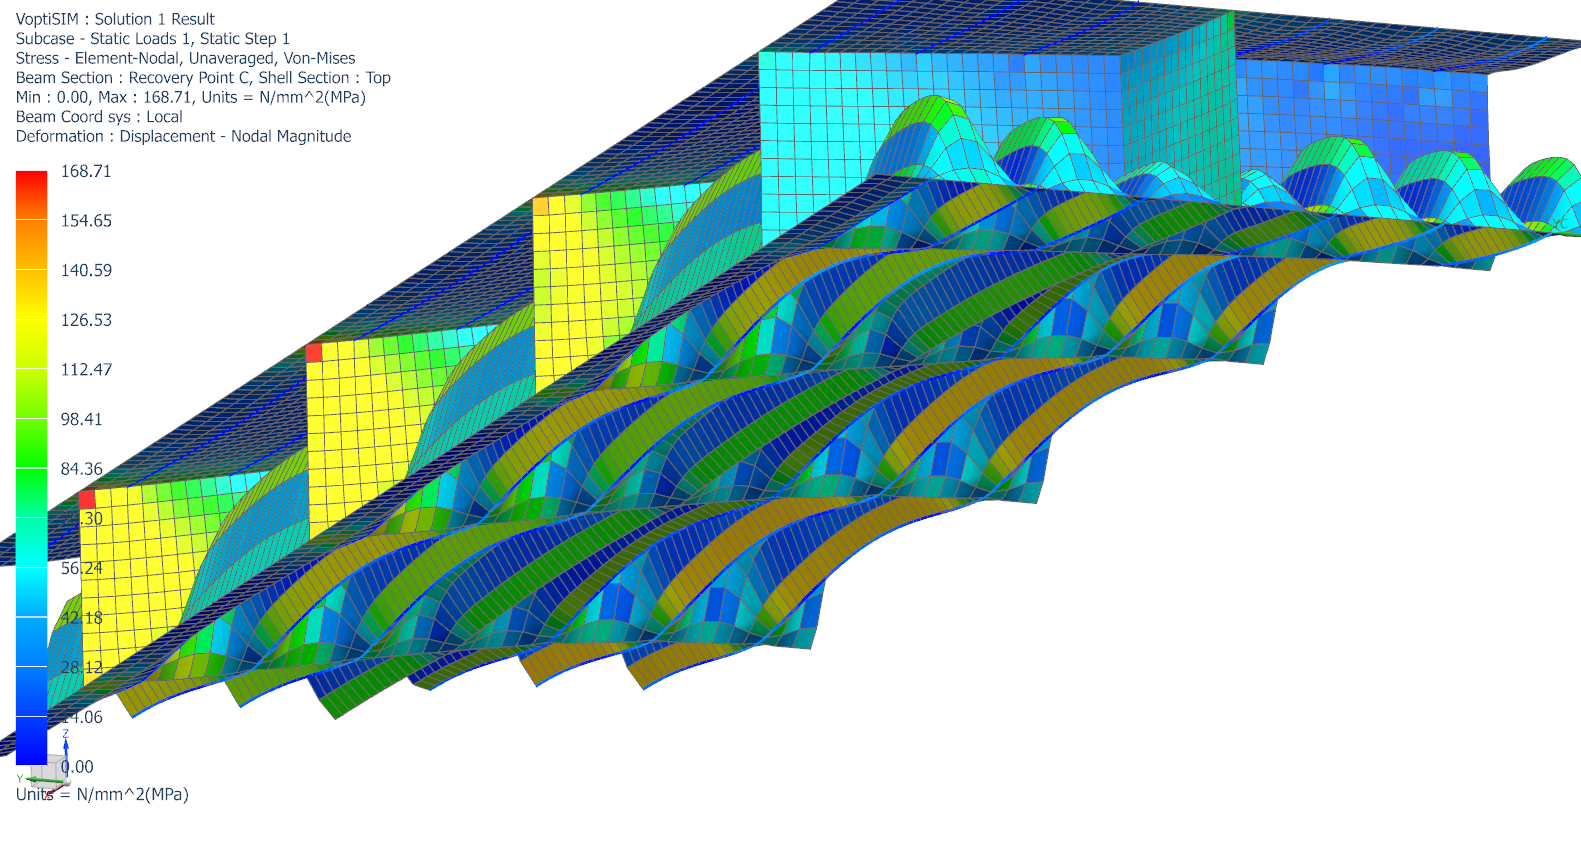
\includegraphics[width=11cm]{fig/VoptiSIM.png}
     \caption{Tensiones son las de Von Mises del resultado final de la optimización.}
     \label{fig:optimizacion}
 \end{figure}

\section{Conclusión}
Terminado el proceso de optimización, queda el trabajo de contrastarlo con resultados de la realidad o con bilbiografía. Se invitan futuros ingenieros a comparar los resultados obtenidos con las curvas de Schade\citep{dominguez1969calculo}. Se puede también continuar el trabajo de reafinar las secciones de las longitudinales pues no dejan de estar sobredimensionadas, incluso después de optimización. 

Con esto dicho, el resultado predispone de buenas caracteristicas. Se pueden observar campos de tensiones en el doble fondo (figura \ref{fig:optimizacion}) similares a la de una placa empotrada (figura \ref{fig:VMempotrado}). Se tiene también un pequeño relieve de tensiones en su cara central. Esto se debe a que los longitudinales no son perfectamente rigidos y aportan un pequeño giro a la placa. Se tiene entonces una superposición con el caso mencionado anteriormente, y el estado de tensiones de una placa simplemente apoyada (figura \ref{fig:VMapoyado}).

En conclusión, un estudio preliminar básico puede ayudar inmensamente llegado al final de un informe, como hemos visto. Se ahorró la necesidad de comparar resultados gracias a la semejanza de placas planas con cascaras.




\bibliography{labibliografia} % Indica archivo
\bibliographystyle{plainnat} 

\end{document}